\documentclass[french]{article}
\usepackage[T1]{fontenc}
\usepackage[utf8]{inputenc}
\usepackage{kpfonts}
\usepackage{babel}
\usepackage{microtype}
\usepackage{graphicx}
\begin{document}

\section{Préambule}
Ce document vise à présenter les études qui ont été menées en lien avec 
la manipulation de données spatiales dans le cadre du projet OSSIA.

Il existe trois défis majeurs : la conception d'un modèle de données générique et assez puissant pour couvrir les cas que nous allons présenter, la représentation graphique de ces données lorsqu'un grand nombre de contrôles sont présents, et le contrôle et l'édition par l'utilisateur.

% (citer tuiles).
% Mettre en parallèle les différentes possibilités d'ffichage d'objets : dans différents plans, en parallèle, etc...
% Possibilité myriam ?
Nous analyserons plusieurs types de projets différents dans lesquels une notion
de contrôle spatial existe, et qui sont utiles à la spécification des besoins.

Puis, nous verrons des solutions possibles pour en permettre un contrôle efficace.

\section{Exemples}
Les exemples sont répartis en trois catégories : ceux liés aux problématiques spatiales dans un contexte sonore et musical, ceux liés aux conceptions d'interfaces, et un cas de contrôle robotique.

\subsection{Cadre sonore}
La spatialisation en musique est une pratique très courante et une recherche importante a eu lieu sur ce sujet.

Il existe deux problèmes distincts et parfois rammenés sous la même égide de spatialisation : 
\begin{itemize}
\item La composition du son avec des composantes spatiales : conception de trajectoires, etc. (citer livre Trajectoires en Musique Électro-acoustiques + livre de Bertrand Merlier.)
\item Le rendu avec un ensemble de hauts-parleurs ou au casque (HRTF, etc.).
\end{itemize}

C'est le premier aspect qui nous intéresse ici. 
Il existe deux fonctionnements possibles, l'un plus adapté au monde de la musique et l'autre au monde de la muséographie. 


\subsubsection{Trajectoires sonores}
Dans un cadre musical, on aura tendance à composer par pistes, et donc à vouloir spatialiser piste par piste. Des objets sonores seront disposés dans un séquenceur tel que Pro Tools ou Reaper, puis, au moment de la composition ou bien lors d'une interprétation en concert, les différentes pistes sont envoyées sur différents canaux audio.

\begin{figure}
\centering
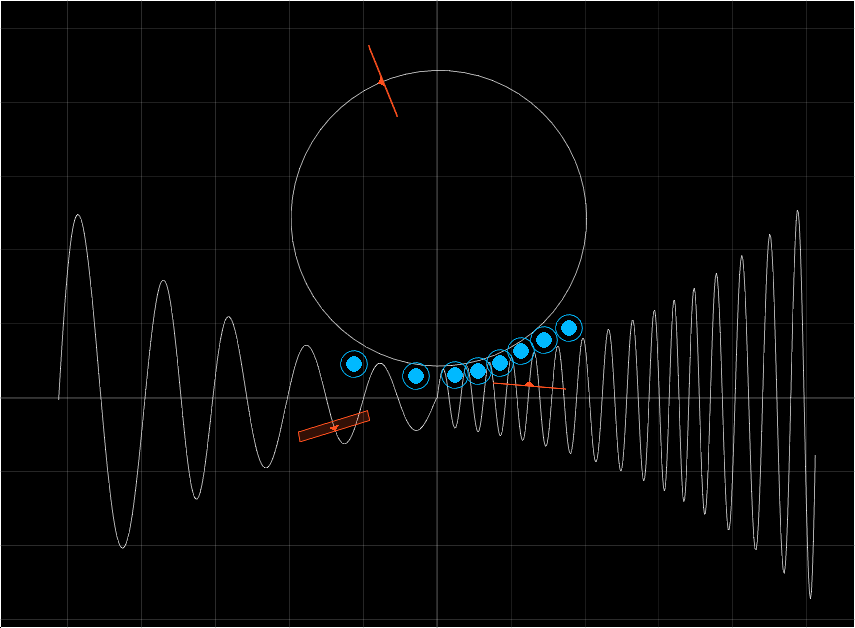
\includegraphics[scale=0.3]{images/iannix.png}
\caption{Une partition composée de trajectoires et de triggers dans le séquenceur graphique IanniX}
\end{figure}



\subsubsection{Positionnement d'objets sonores}
Dans un cadre muséographique, on a plus souvent des objets sonores qui peuvent être associés à des éléments graphiques : des notes dans un manuscrit, un personnage sur un tableau... On désire alors contrôler le comportement de cet objet sonore au fil du temps et le scénariser, le faire se déplacer, etc.

Cette approche est aussi plus pertinente dans un cadre vidéo-ludique : en effet, les outils de conception de jeu-vidéo (citer partie rapport cnam) ont une approche fortement orientée objet - la méthode actuellement la plus répandue dans l'industrie est celle des Entity Component Systems %todo source
, qui permet d'appliquer différentes couches applicatives (qui peuvent contenir des données, des comportements...) à un objet du jeu, comme un ennemi.

Voici plusieurs examples d'applications :
\paragraph{Application 1 : Sonopluie}
Ici, des utilisateurs font un parcours dans une ville. Ils ont un casque et sont géolocalisés. En fonction de leur position et de leur parcours, ils entendent des messages rappelant des évènements historiques de la ville. 

De plus, si des utilisateurs se croisent, l'application peut en avoir conscience et déclencher des évènements spécifiques.

Cette application a plusieurs pré-requis : 
\begin{itemize}
\item L'outil de conception doit, au minimum, permettre de placer des points sur une carte et de définir une action sur le périphérique de l'utilisateur, lorsqu'il rencontre un point.
\item Pour plus de richesse, des zones sonores peuvent être définies : par exemple, une bande de plage.
\item Il doit y avoir une notion de scénarisation telle qu'offerte par i-score, permet de construire une histoire au cours du temps, plutôt que de simplement avoir une liste de hot-spots interactifs.
\item Enfin, se pose la question de la répartition et de l'interaction entre plusieurs protagonistes. Une possibilité serait de définir des zones d'interactions qui ne s'activent que lorsque plusieurs participants sont présents à l'intérieur. Les périphériques des utilisateurs présents dans cette zone doivent communiquer entre eux (ou bien communiquer via un serveur, mais cela nécessite des appareils possédant une connection internet).
\end{itemize}

\paragraph{Application 2 : Le promeneur écoutant}

cf. rapport CNAM 


\subsection{Cadre IHM}
Ici, nous nous intéressons aux possibilités de création et de contrôle dynamique d'interfaces graphiques. La plupart des paradigmes d'UI permettent de définir des vues dans un éditeur graphique, mais ces vues sont en général statiques et il est nécessaire de recourir à des langages de programmation pour avoir une évolution dans le logiciel \textit{(à vrai dire il y a des outils graphiques pour ça dans Qt par exemple, j'imagine que ça doit pouvoir se faire assez bien dans Flash aussi ?)}. 

Problématiques : création d'objet ??

Pb. de l'interface d'animation (gestion du temps, tweens ,etc.)

Comportements de masse / comportements aléatoires ?

\subsubsection{Contrôle d'interfaces utilisateurs}
Le premier cas est celui d'une application en mode kiosque, possédant un menu de choix des langues, qui mène pour chaque langue à un menu principal permettant de choisir des vidéos à lire en mosaïque.

Lorsqu'une langue est choisie, l'écran principal glisse depuis la droite. Les boutons ont une animation lorsqu'ils sont pressés. Lorsqu'une vidéo est pressée, elle se met en lecture. Des \textit{gestures} permettent de déplacer les vidéos, en suivant des lois de physique basiques (notamment, les vidéos peuvent tourner et rentrer en collision).

(\textit{note:  s'il y a une vraie application muséo à la place ici je suis preneur :) j'ai juste imaginé des choses pour faire un example.})

Les problématiques, ici, sont : 
\begin{itemize}
\item Le contrôle d'un grand nombre d'élements statiques, et la hiérarchisation de ces éléments. Par exemple, si les boutons de langues sont enfants du premier menu, on veut qu'ils suivent le déplacement de leur menu parent.
\item Un questionnement sur les modèles physiques. Cela a déjà été abordé pour les modèles masse-ressort évoqués en spatialisation de musique %TODO.
\item La gestion d'animations. Généralement, une animation consiste en l'interpolation de paramètres dans le temps, en passant par des états prédéfinis (keyframes).
\end{itemize}

\subsubsection{Navigation dans espaces de paramètres}
Un problème plus général est celui de la gestion des espaces de paramètres particuliers.

Par exemple, pour choisir et animer la couleur d'un élément dans le temps, il est nécessaire d'avoir des outils de création adaptés, tout en gardant les primitves de trajectoires et d'objets évoquées précédemment.

Un second point est celui de la gestion des correspondances entre espaces de données. Ainsi, si on désire automatiser un point sur un plan en deux dimensions dans le temps, il doit être possible de le faire selon les systèmes de coordonnées cartésiennes ou polaires.

De même, pour les couleurs il est important de pouvoir travailler en RVB, mais aussi en L*a*b*, HSL, et notamment de pouvoir passer facilement d'un mode à l'autre.

Enfin, le dernier point est le cas d'une aide à l'écriture pour une application comportant un grand nombre de paramètres, potentiellement artistiques. Le problème de la visualisation se pose lorsque ces paramètres sont représentés sur une seule dimension : %TODO screenshot iscore

\subsection{Contrôle de robots}
Une application intéressante est celle des chorégraphies de robot. Ce chantier, commencé en 2015, vise à étendre les possibilités du séquenceur i-score d'abord à des robots quadrupèdes Metabots, puis, potentiellement à des drones.

Là encore, la question de l'écriture se pose, et notamment le cas de la gestion d'un grand nombre d'objets dans un espace relativement restreint.

De plus, ces objets ne vont pas forcément réagir comme prévu : si par exemple un robot est programmé pour aller tout droit, mais qu'il rencontre un autre robot qui serait tombé en panne sur le chemin, actuellement le premier robot ne saurait en tenir compte et rentrerait en collision avec le second robot.


\section{Réalisations}
\subsection{État de l'art sur méthodes spatiales, positionnement, trajectoires}

\subsubsection{Free-hand drawing sur tableau}
À titre d'exemple pour des démonstrations et exposés, un outil permettant de dessiner des zones de manières arbitraire sur un tablea a été développé. % TODO screenshot

\subsubsection{Liste des tâches et prototype pour processus de mapping spatial}
Suite aux différents cas d'utilisation qui ont été présentés, un état de l'art a été effectué dans le domaine de l'authoring spatial, et des techniques et méthodes possibles.

- 


\subsection{Clients manipulant des données spatiales}
\subsubsection{Interopérabilité avec Qt}
Un plug-in pour i-score permettant d'exposer l'arbre d'objets d'une application Qt a été développé. Cela permet de contrôler facilement la position et le contenu des éléments d'une interface graphique réalisée avec cette technologie depuis i-score.

\subsubsection{Contrôle d'OpenAL}
OpenAL est une bilbiothèque ayant été développée pour les besoins des jeux vidéos au début des années 2000. Elle se base sur une notion de sources sonores associées à des fichiers sons, qui sont positionnées en trois dimensions, ainsi que d'un listener qui se déplace et perçoit donc les sons plus ou moins forts. Une implémentation récente, OpenAL-soft, permet d'utiliser des HRTF pour avoir une sensation de spatialisation réaliste au casque.  

Un outil exposant des sources OpenAL via le protocole Minuit et permettant de charger des sons, puis de les positionner dans l'espace a été implémenté. Ces sources sont donc contrôlables depuis i-score.

\subsubsection{Contrôle de metabots}
Une couche de communication entre i-score et les robots metabot %TODO photo
a été développée et a mené à une présentation aux Robot Makers Day, avec notamment 
une chorégraphie ou deux robots sont contrôlés et synchronisés musicalement avec i-score. 

Cela a été l'occasion de comparer le développement d'une chorégraphie entre i-score, et 
un langage de programmation graphique inspiré de Scratch. Les résultats ont été probants : il a fallu 
beaucoup moins de temps pour produire une même chorégraphie dans i-score que dans l'autre langage.

\section{Conclusion}

Problèmes restants : question de visualisation / rendu, etc.

\end{document}